\chapter{Modeling}\label{ch:modeling}


In order to understand the behaviour of the system, a mathematical model followed by a simulation had to be done. 

\section{DC motors dynamics model} \label{dc_math}

\begin{table}[h]
\centering
\begin{tabular}{cccll}
\hline
Parameter                   & Description                               & Nominal Value                                 &  &  \\ \hline
\multicolumn{1}{|c|}{K}     & \multicolumn{1}{c|}{Motor constant}       & \multicolumn{1}{c|}{0.1838 V/(rad/s)  Nm/amp} &  &  \\ \cline{1-3}
\multicolumn{1}{|c|}{R}     & \multicolumn{1}{c|}{Armature resistance}  & \multicolumn{1}{c|}{11.5 $\Omega$}            &  &  \\ \cline{1-3}
\multicolumn{1}{|c|}{L}     & \multicolumn{1}{c|}{Armature inductance}  & \multicolumn{1}{c|}{0.1 H}                    &  &  \\ \cline{1-3}
\multicolumn{1}{|c|}{$J_r$} & \multicolumn{1}{c|}{Rotor inertia}       & \multicolumn{1}{c|}{0}                        &  &  \\ \cline{1-3}
\multicolumn{1}{|c|}{$b_r$} & \multicolumn{1}{c|}{Rotor damping}        & \multicolumn{1}{c|}{0.0221}                   &  &  \\ \cline{1-3}
\multicolumn{1}{|c|}{$J_w$} & \multicolumn{1}{l|}{Load inertia} & \multicolumn{1}{c|}{2.8033e-5 $KgM^2$}        &  &  \\ \cline{1-3}
\multicolumn{1}{|c|}{n}     & \multicolumn{1}{c|}{Gear ratio}           & \multicolumn{1}{c|}{1:48}                     &  &  \\ \cline{1-3}
\multicolumn{1}{l}{}        & \multicolumn{1}{l}{}                      & \multicolumn{1}{l}{}                          &  &  \\ \hline
\end{tabular}
\caption{Motor parameters}
\label{my-label}
\end{table}

\missingfigure{We need a figure right here!}

This section describes the dynamic mathematical model of the DC motors, including moment of inertia, torque and friction. In a DC motor the produced electromagnetic torque($\boldsymbol{T_e}$) is linearly proportional to the armature current and the magnetic field. If we assume that the magnetic field is constant, the torque is only proportional to the armature current(\textbf{I}) and the torque constant($\boldsymbol{K_t}$) as evident in equation \ref{eq1}. \\

\begin{equation} \label{eq1} 
T_e = IK_t
\end{equation}

The back electromotive force voltage($E_b$) is proportional to the angular velocity($\omega$) of the shaft times the Back emf constant($K_b$).(Equation \ref{eq2})

\begin{equation} \label{eq2}
E_b = \omega K_b
\end{equation}

Because the two constants $K_t$ and $K_b$ are equal in SI units, in further equations and simulations they will be denoted only as a motor constant $K$.

\begin{equation} \label{eq3}
K_t = K_b = K
\end{equation} 

Furthermore, from figure \todo{reference to figure}, using Kirchhoff's voltage law, we can derive the equations governing the electrical part of the DC motor, where the applied voltage (\textbf{V}) is proportional to the voltage drop through the armature resistance(\textbf{R}) and inductance(\textbf{L}), and the back electromotive voltage($\boldsymbol{E_b}$). \ref{eq4}

\begin{equation} \label{eq4}
V = RI + L\frac{dI}{dt} + E_b
\end{equation} 

The mechanical part of the DC motor(mechanical part of figure \todo{reference to figure}) is derived from the equations, where the mechanical torque($\boldsymbol{T_m}$) is the difference between the electromagnetic torque($\boldsymbol{T_e}$) and the rotational losses ($\boldsymbol{T_b}$). \ref{eq5}

\begin{equation} \label{eq5} 
T_m = T_e - T_b
\end{equation} 

Using Newton's second law for rotational motion and substituting from equation\ref{eq1}, we can rewrite equation \ref{eq5} as:

\begin{equation} \label{eq6}
J\dot{\omega} = KI - b\omega
\end{equation}

Where \textbf{J} is the load's inertia and \textbf{b} is the viscous friction in the motor's bearings.
Further substitution in equation \ref{eq4} with the derived back emf from \ref{eq2} results in:

\begin{equation} \label{eq7}
V = RI + L\frac{dI}{dt} + K\omega
\end{equation}

Equations \ref{eq6} and \ref{eq7} are the combined equations of motion for the DC motor.

Applying the Laplace transform to the equations, we can derive the transfer function of the DC motor.

\begin{align}  
sJ\Omega(s) + b\Omega(s) = KI(s) \label{eq8}\\
sLI(s) + RI(s) = V(s) - K\Omega(s) \nonumber
\end{align}

\begin{center}
$\Downarrow$
\end{center}

\begin{align} 
\frac{\Omega(s)(sJ + b)}{K} = I(s) \label{eq9} \\
I(s)(sL + R) + K\Omega(s) = V(s)  \nonumber 
\end{align}

Substituting with \textbf{I(s)} in the second part of equation \ref{eq9}, and setting the angular velocity($\boldsymbol{\Omega(s)}$) as output and the voltage (\textbf{V(s)}) as input results in the transfer function for the DC motor.(\ref{eq10})

\begin{equation} \label{eq10}
\frac{\Omega(s)}{V(s)} = \frac{K}{(Js + b)(sL + R) + K^2}
\end{equation}

\subsection{Simulink Model} \label{dc_model}

In this subsection, the previously derived equations are represented in a block diagram using Matlab's Simulink environment. There are several possible ways to arrange the blocks governing the DC motor, thus in this paper a familiar approach is considered.

\begin{table}[h]
\centering
\begin{tabular}{cccll}
\hline
Parameter                   & Description                               & Nominal Value                                 &  &  \\ \hline
\multicolumn{1}{|c|}{K}     & \multicolumn{1}{c|}{Motor constant}       & \multicolumn{1}{c|}{0.1838 V/(rad/s)  Nm/amp} &  &  \\ \cline{1-3}
\multicolumn{1}{|c|}{R}     & \multicolumn{1}{c|}{Armature resistance}  & \multicolumn{1}{c|}{11.5 $\Omega$}            &  &  \\ \cline{1-3}
\multicolumn{1}{|c|}{L}     & \multicolumn{1}{c|}{Armature inductance}  & \multicolumn{1}{c|}{0.1 H}                    &  &  \\ \cline{1-3}
\multicolumn{1}{|c|}{$J_r$} & \multicolumn{1}{c|}{Rotor inertia}       & \multicolumn{1}{c|}{0}                        &  &  \\ \cline{1-3}
\multicolumn{1}{|c|}{$b_r$} & \multicolumn{1}{c|}{Rotor damping}        & \multicolumn{1}{c|}{0.0221}                   &  &  \\ \cline{1-3}
\multicolumn{1}{|c|}{$J_w$} & \multicolumn{1}{c|}{Load inertia} & \multicolumn{1}{c|}{2.8033e-5 $KgM^2$}        &  &  \\ \cline{1-3}
\multicolumn{1}{|c|}{n}     & \multicolumn{1}{c|}{Gear ratio}           & \multicolumn{1}{c|}{1:48}                     &  &  \\ \cline{1-3}
\multicolumn{1}{l}{}        & \multicolumn{1}{l}{}                      & \multicolumn{1}{l}{}                          &  &  \\ \hline
\end{tabular}
\caption{Motor parameters}
\label{motor_par}
\end{table}

As evident from equation \ref{eq10}, the voltage is the input of the system, while the angular velocity is the output. In order to accurately apply the equations, while attaining the desired result, a modification of equations \ref{eq6} and \ref{eq7} was made.(\ref{eq11})

\begin{align}
\frac{dI}{dt} = \frac{1}{L}(V - RI - K\omega)\label{eq11} \\
\frac{d\omega}{dt} = \frac{1}{J}(KI - b\omega) \nonumber
\end{align}

The block diagram representation in figure \ref{fig::dcmfigure} has the integrals of the rotational acceleration and the rate of change of the armature current considered as outputs based on equations \ref{eq11}.

\begin{figure}[h]
\centering
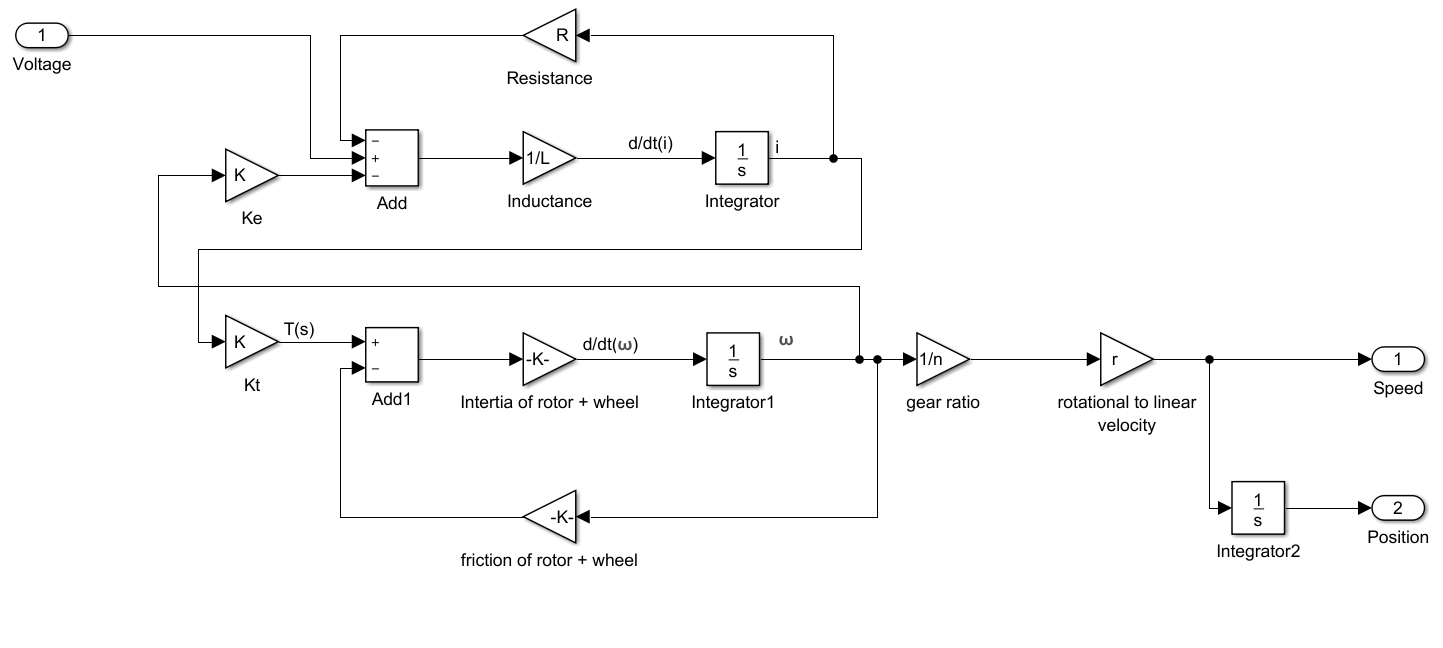
\includegraphics[width=1.1\textwidth]{dc_motorD}
\caption{DC Motor Block Diagram}
\label{fig::dcmfigure}
\end{figure}

The inclusion of the gear ratio (\textbf{n}) and the radius of the wheel (\textbf{r}) products to the angular velocity in the end of the block diagram, results in model scaling for the linear velocity (\textbf{v}) of the wheel. (\ref{eq12})

\begin{equation} \label{eq12}
v = r\omega
\end{equation}

Performing integration on the derived linear velocity results in obtaining the linear displacement of the wheels, later to be used with the kinematics model. 

To summarise, the goal was to relate the voltage to the speed. The input of the block diagram is the voltage of the motor (\textbf{V}) while the outputs are the linear speed caused by wheel rotation and the linear displacement, obtained from integrating the speed. The blocks comprising the upper and lower part of the block diagram, directly correspond to equation \ref{eq11} (upper part correspond to the electrical part of the motor; lower part correspond to the mechanical part of the motor).

Furthermore, as this paper is concerned with the development of a differential drive robot, the block diagram in figure \ref{fig::dcmfigure} is solely a subsystem of the complete kinematics model. That is, two DC motor subsystems are required in order to describe the complete motor/wheel dynamics. 

\section{Kinematics Model of Differential Drive}

Differential drive is a common mechanism in mobile robotics. It consists of two wheels on a common axis, driven by two motor, where each wheel can be independently driven in either forward or backward direction. That is, by varying the velocities of each wheel, different  trajectories could be achieved. Importantly, the rotation the robot performs is based on a point common to the right and left wheel axis, denoted as Instantaneous Center of Curvature(\textbf{ICC}). The kinematic representation can be observed in figure \ref{fig::diff_drive_over} .

\begin{figure}[h]
\centering
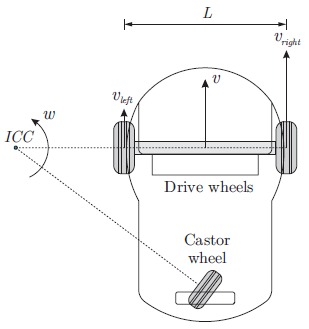
\includegraphics[width = 0.5\textwidth]{Kinematics_char}
\caption{Differential drive overview}
\label{fig::diff_drive_over}
\end{figure}

The linear speed, previously derived from chapter \ref{dc_model}, is represented as $v_r$ and $v_l$, for each of the wheels. The speed of the robot is taken as the average speed of each wheel.

\begin{equation} \label{eq13}
v = \frac{v_r + v_l}{2} 
\end{equation}

The angular speed of the robot (or turning speed) is based on the linear speeds of each wheel and the distance between the wheels. It is denoted as \textbf{W} in equation \ref{eq14}.(not to be confused with $\omega$, the rotational speed of the motor)

\begin{equation} \label{eq14}
W = \frac{v_r - v_l}{l}
\end{equation}

The relation between the linear speed and the angular speed of the robot is similar to equation \ref{eq12}.

\begin{equation} \label{eq15} 
v = WD
\end{equation}

Where D is the turning radius, from the midpoint of the wheels to the ICC. Solving for the turning radius, yields:

\begin{align}
D = \frac{v}{W} \label{eq16} \\
= \frac{l}{2}\frac{v_r + v_l}{v_r - v_l} \nonumber
\end{align}

Analysis of the above equation leads to the consideration of three cases where certain behaviour is to be expected.

\begin{itemize}

\item $\boldsymbol{v_r = v_l}$ \\ In this case scenario, both wheels have the same speed. The robot's speed from equation \ref{eq13} is simply equal to the individual speed of each of wheel. On the other hand, the angular speed from equation \ref{eq14} becomes 0, and the turning radius infinite. The robot is expected to perform straight linear motion.

\item $\boldsymbol{v_r = 0}$ or $\boldsymbol{v_l = 0}$ \\ In this case scenario, the turning radius becomes $\frac{l}{2}$. The robot is expected to perform rotation either about the right or the left wheel, with the center of rotation being the zero velocity wheel. 

\item $\boldsymbol{v_l = -v_r}$ \\ In this case scenario, the turning radius and the linear speed become 0, while the angular speed is doubled. The robot is expected to perform rotation about it's midpoint, or simply put in-place rotation.

\end{itemize}

It is important to mention that the wheels , present in the system , carry some \textbf{nonholonomic} constraints. That is, the robot's local movements are restricted, while no restrictions are present in the global navigation. We can further extend the idea with the use of generalised coordinates.

\begin{equation} \label{eq17}
q = (x,y,\theta) 
\end{equation}

Equation \ref{eq17} could be seen as a point on a two dimensional Cartesian coordinate system, where x and y are the axis and $\theta$ is the angle between the x axis and the point. 

Figure \ref{fig::orientation} shows the robot representation based on the generalised coordinates.

\begin{figure}[h]
\centering
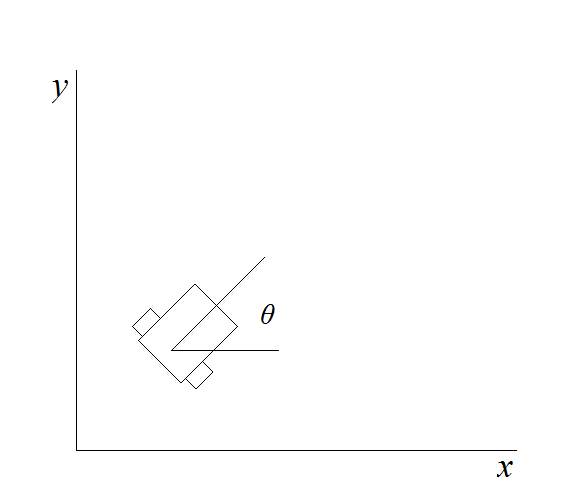
\includegraphics[width = 0.4\textwidth]{Orientation_xy}
\caption{Robot representation in Cartesian coordinates}
\label{fig::orientation}
\end{figure}

We can picture the constrains for the wheels by setting the sideways velocity to zero. That is, the robot can not perform sideways movements like slipping or sliding, but is not limited from manoeuvring in that position, whatsoever. 

\begin{equation} \label{eq18}
\dot{x}sin(\theta) - \dot{y}cos(\theta) = 0
\end{equation}

Equation \ref{eq18} is a common nonholonomic constraint in mobile robotics. \todo{reference to the caltech report}

Particularly if the robot is viewed as a point, the Kinematics equations in Cartesian space can be derived as:

\begin{align}
\dot{x} = vcos(\theta) \nonumber \\
\dot{y} = vsin(\theta) \label{eq19} \\
\dot{\theta} = \omega  \nonumber 
\end{align}

In the case of a differential drive robot, substitution of the linear and angular velocities, \textbf{v} and $\boldsymbol{\omega}$, with the previously derived in equation \ref{eq13} and \ref{eq14} average robot speed and angular robot speed (with respect to the center of rotation between the wheels), will results in the kinematics equations for locomotion of a differential drive. 

\begin{align}
\dot{x} = \frac{v_r + v_l}{2}cos(\theta) \nonumber \\
\dot{y} = \frac{v_r + v_l}{2}sin(\theta) \label{eq20} \\
\dot{\theta} = \frac{v_r - v_l}{l} \nonumber
\end{align}

In equation \ref{eq20} we will have a change in the robot's position (x,y,$\theta$) when the velocity of each wheel is controlled. 

\subsection{Kinematics in simulink} 

\begin{table}[h]
\centering
\begin{tabular}{cccll}
\hline
Parameter                   & Description                               &  &  \\ \hline
\multicolumn{1}{|c|}{l}     & \multicolumn{1}{c|}{Distance between wheels}       &  &  \\ \cline{1-2}
\multicolumn{1}{|c|}{$v_r$} & \multicolumn{1}{c|}{Linear speed of right wheel}  &  &  \\ \cline{1-2}
\multicolumn{1}{|c|}{$v_l$} & \multicolumn{1}{c|}{Linear speed of left wheel}  &  &  \\ \cline{1-2}
\multicolumn{1}{|c|}{v}     & \multicolumn{1}{c|}{Average linear robot speed}  &  &  \\ \cline{1-2}
\multicolumn{1}{|c|}{W}     & \multicolumn{1}{c|}{Angular robot speed}        &  &  \\ \cline{1-2}
\multicolumn{1}{|c|}{D}     & \multicolumn{1}{c|}{Turning radius}         &  &  \\ \cline{1-2}
\multicolumn{1}{l}{}        & \multicolumn{1}{l}{}                      &  &  \\ \hline
\end{tabular}
\caption{Kinematics parameters}
\label{kin_para}
\end{table}

Using equations \ref{eq13} and \ref{eq14} a simulink block diagram is constructed in figure \ref{fig::diff_simulink}.

\begin{figure}[h]
\centering
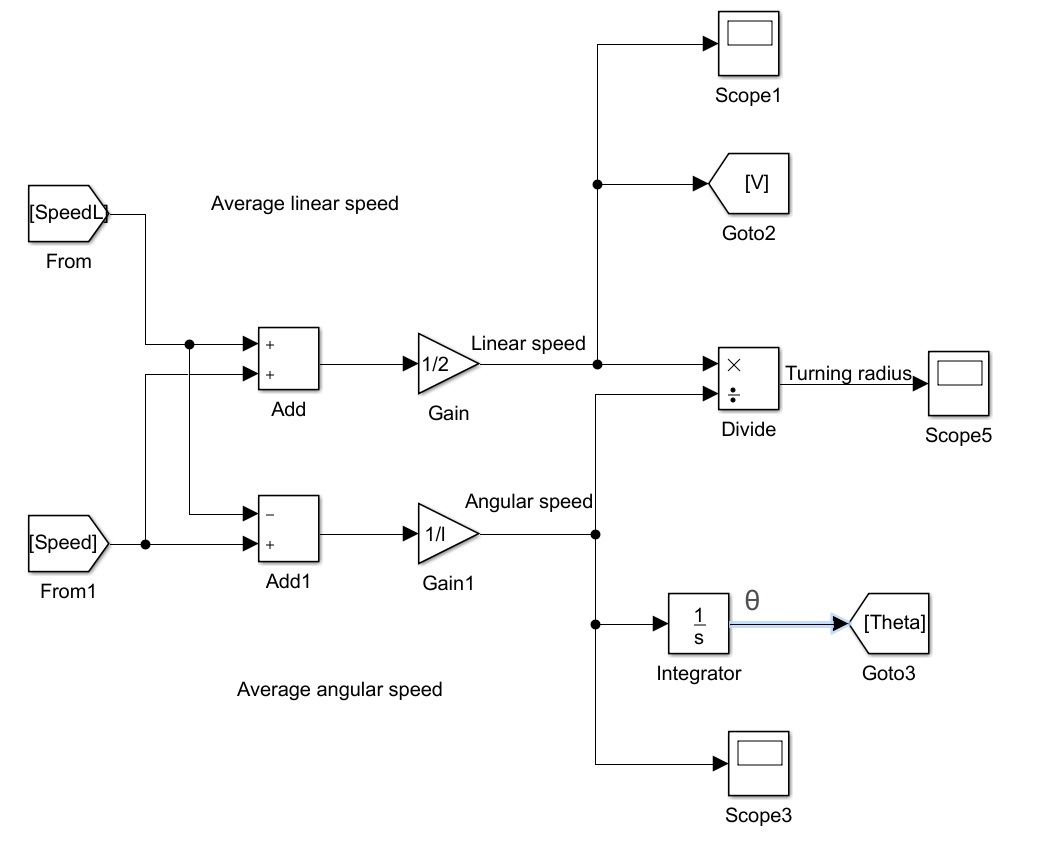
\includegraphics[width = 0.8\textwidth]{diff_drive_kin_simulink}
\caption{Differential drive kinematics}
\label{fig::diff_simulink}
\end{figure} 

The inputs are the individual wheel velocities, arranged to reflect the previously mentioned equations. The middle output is the turning radius \textbf{D}, which is governed by equation \ref{eq16}. The derived average linear speed is to be further used in equation \ref{eq20} to estimate the position of the robot based on it's angle through time, where the angle ($\theta$) is   obtain from integrating $\dot{\theta}$, which itself is the angular speed of the robot. 

\begin{figure}[h]
\centering
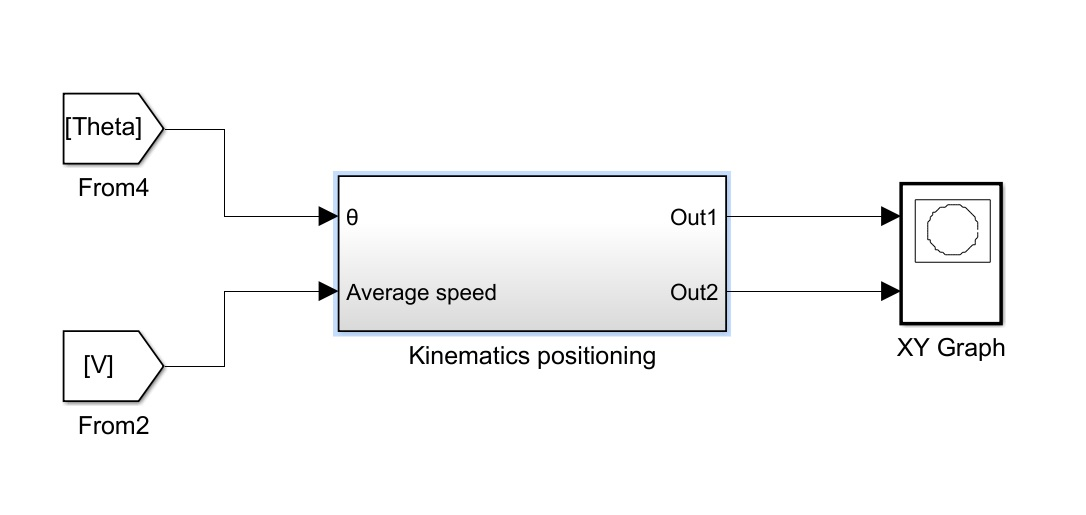
\includegraphics[width = 0.8\textwidth]{kin_pos_subsystem}
\caption{Positioning subsystem}
\label{fig::pos_sub}
\end{figure} 

In figure \ref{fig::pos_sub} the inputs are the the average speed and the orientation of the robot, while the outputs X and Y from equation \ref{eq20} are fed in a graph to observe the robot's trajectory through time. 

\begin{figure}[h]
\centering
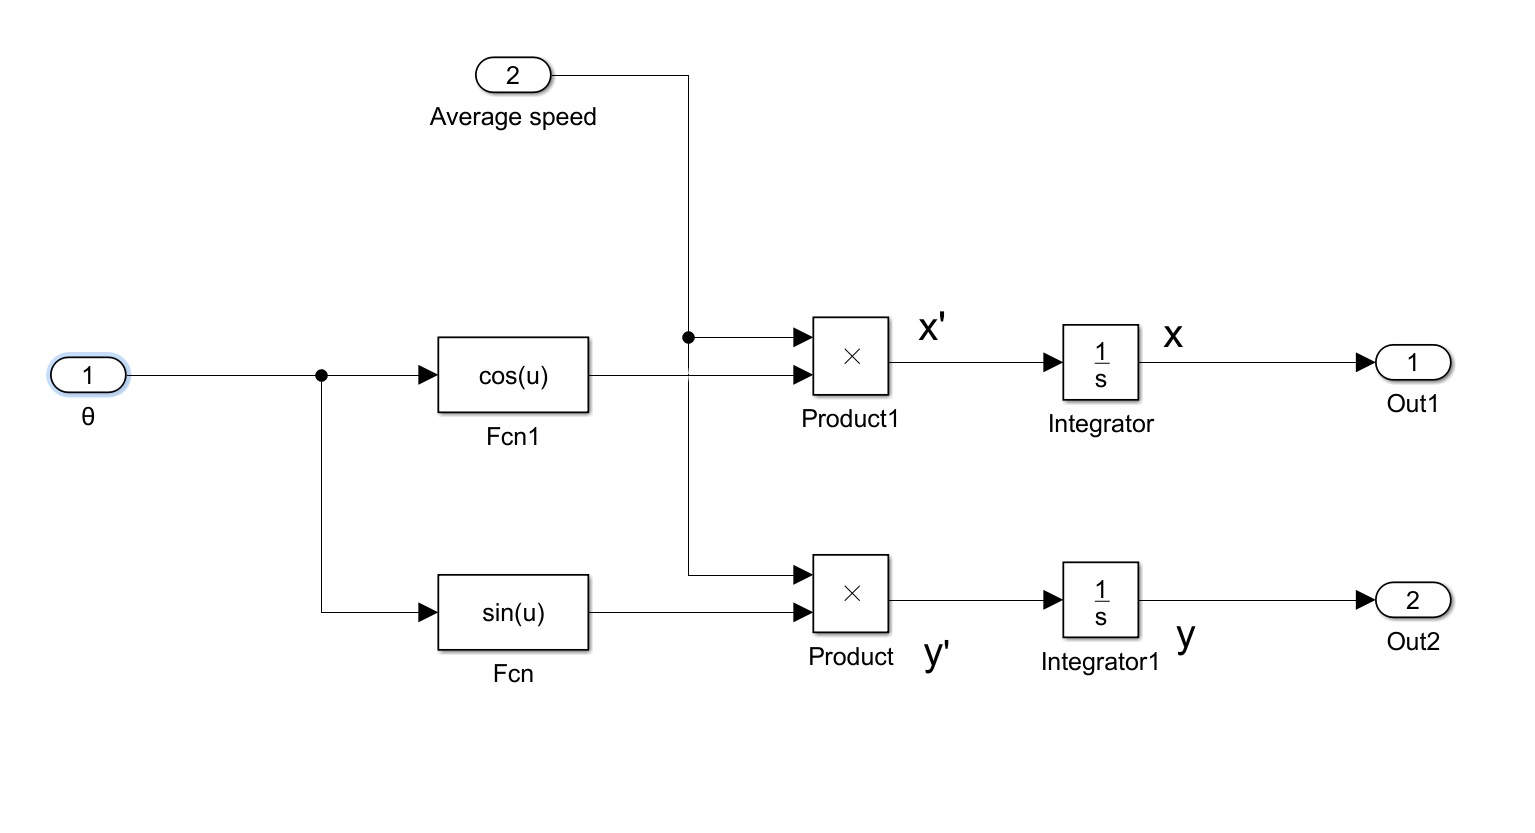
\includegraphics[width = 0.8\textwidth]{kin_model_pos}
\caption{Positioning subsystem}
\label{fig::pos_model}
\end{figure} 

The subsystem from figure \ref{fig::pos_sub} is composed of blocks arranged to reflect equation \ref{eq20}. The outputs $\dot{x}$ and $\dot{y}$ are further integrated to graph the trajectory of the robot. 

\section{Complete model}